\chapter{Introduction}
\label{ch:introduction}

This chapter motivates the presented research, introduces the central problem of the systematic time-shift anomaly in machine-learned glucose predictions, and defines the three core research objectives. Section~\ref{sec:intro:motivation} describes the underlying clinical context of Type~1 diabetes. Section~\ref{sec:intro:timeshift} explains the time-shift artefact that motivates the ablation study. Section~\ref{sec:intro:scope} defines the scope of the evaluation and states the research questions. Section~\ref{sec:intro:contributions} summarizes the primary scientific contributions, and Section~\ref{sec:intro:structure} details the overall structural organization of the thesis.

% ================================================================
\section{Clinical Motivation}
\label{sec:intro:motivation}
% ================================================================

\begin{planned}
    \item Characterization of Type~1 Diabetes Mellitus as an autoimmune condition involving the complete destruction of endogenous insulin production which necessitates lifelong external insulin administration.
    \item Presentation of global epidemiological data using the IDF Diabetes Atlas to highlight the expanding relevance of the condition and the persistent high risk of acute complications.
    \item Explanation of Continuous Glucose Monitoring technology as a continuous sensor-based measurement tool that provides the foundational input signal for modern automated insulin delivery loops.
    \item Definition of hypoglycemia thresholds and the critical clinical need for early warning mechanisms due to the physiological pharmacodynamic delays of insulin.
    \item Description of Figure 1.1: Visual presentation of a real hypoglycemia episode where the interstitial glucose concentration crosses the critical threshold line during a steep downward trajectory.
\end{planned}

\begin{figure}[htb]
    \centering
    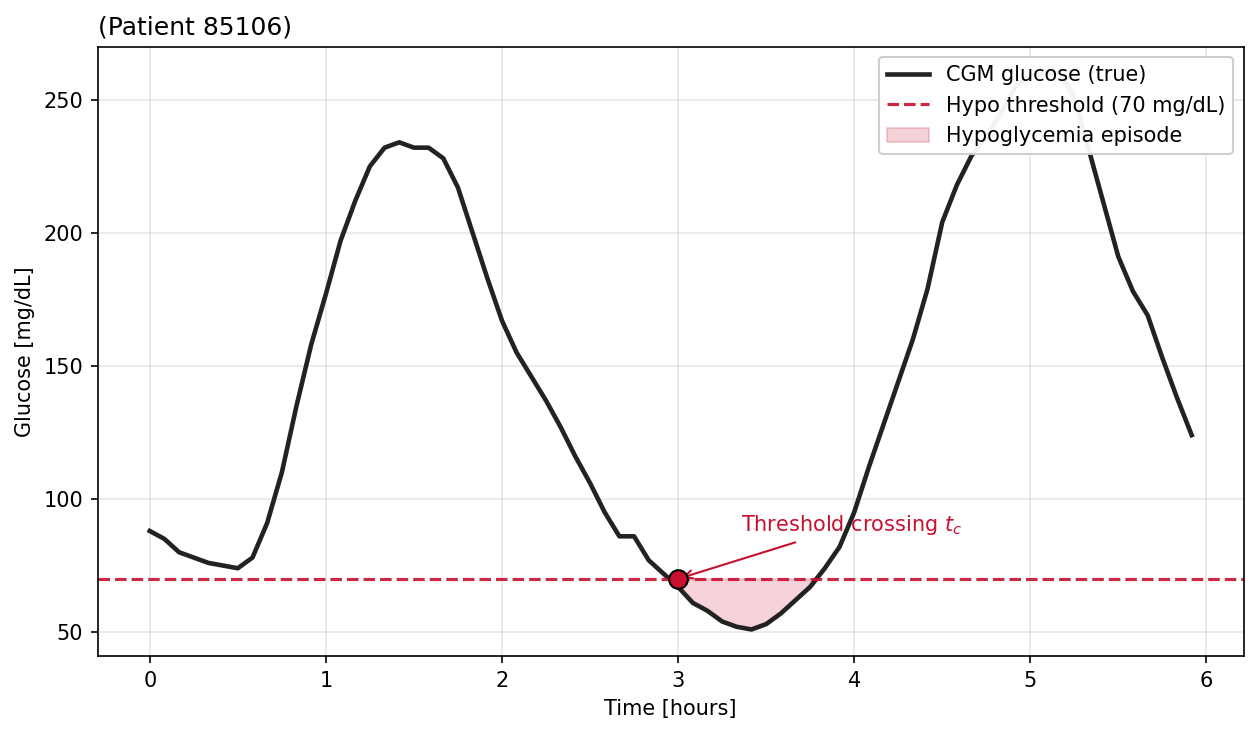
\includegraphics[width=0.9\textwidth]{hypo_episode.png}
    \caption[Typical hypoglycemia episode in a CGM signal]{%
    Typical hypoglycemia episode in the CGM signal of a Type~1 diabetes patient.
    The glucose value drops below the clinical threshold of 70~mg/dL.
    A preventive measure must be initiated already during the downward
    phase, not only after the threshold has been crossed, which motivates
    the need for accurate early-warning systems addressed in this thesis.}
    \label{fig:intro:hypo_episode}
\end{figure}

% ================================================================
\section{The Time-Shift Problem in Glucose Forecasting}
\label{sec:intro:timeshift}
% ================================================================

\begin{planned}
    \item Definition of the systematic time-shift anomaly where standard regression models optimize point-wise criteria but produce predictions delayed by approximately 50 to 55 minutes.
    \item Analysis of the mathematical root cause stemming from the high lag-1 autocorrelation of the univariate glucose signal which induces models to mimic historical states rather than anticipating future trends.
    \item Explanation of the severe clinical consequences of this delay because delayed threshold crossings render forecast-based event detection mechanisms ineffective.
    \item Introduction of the lag\_rmse diagnostic metric as a specialized evaluation tool designed to quantify the specific error component caused by temporal misalignment.
    \item Description of Figure 1.2: Visual comparison between the actual glucose trajectory and a delayed model forecast to demonstrate the shape-preserving but temporally shifted nature of the prediction.
\end{planned}

\begin{figure}[htb]
    \centering
    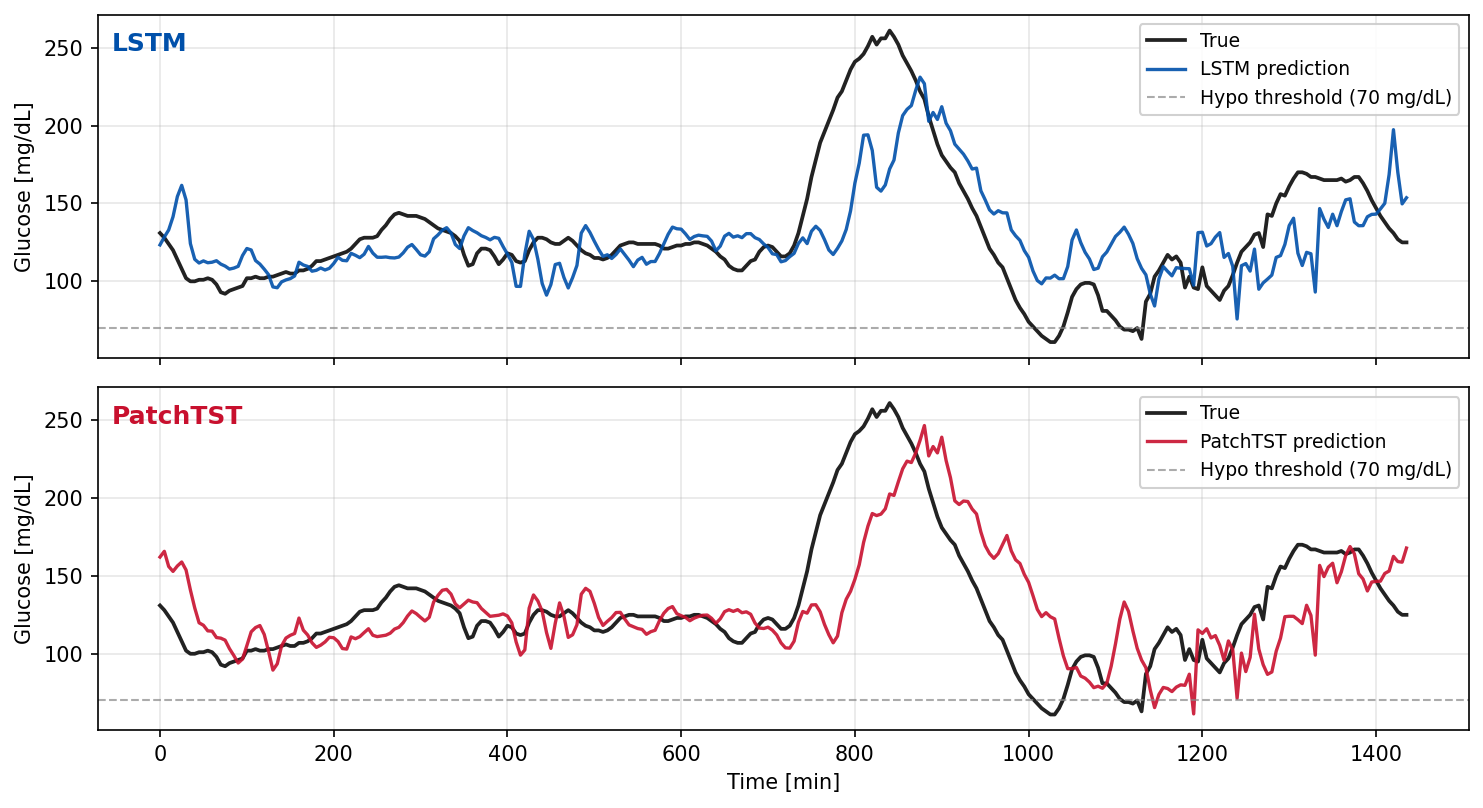
\includegraphics[width=0.9\textwidth]{timeshift_demo.png}
    \caption[Illustration of the time-shift artefact in glucose forecasting]{%
    Illustration of the time-shift artefact in MSE-trained univariate
    glucose forecasting models. Both the LSTM (top) and PatchTST (bottom)
    predictions follow the true glucose trajectory closely in shape but
    are delayed by approximately 55~minutes. Hypoglycemia threshold
    crossings are therefore detected too late, or not at all, which
    motivates the lag\_rmse diagnostic metric introduced in this thesis.}
    \label{fig:intro:timeshift_demo}
\end{figure}

% ================================================================
\section{Scope and Research Questions}
\label{sec:intro:scope}
% ================================================================

\begin{planned}
    \item Overview of the T1DATA clinical dataset consisting of continuous glucose monitoring records from 36 anonymized patients over multiple weeks.
    \item Justification for the strictly univariate modeling approach to deliberately isolate the temporal predictive capacity of the glucose signal itself without confounding external inputs.
    \item Selection rationale for the two evaluated network architectures: the recurrent Long Short-Term Memory network and the patch-based PatchTST Transformer model.
    \item Description of the controlled ablation design framework where exactly one configuration variable is altered per objective while all underlying hyperparameters remain constant.
    \item Formal presentation of the three central research questions regarding the impact of offset-aware loss functions, multi-step output strategies, and direct binary event classification.
\end{planned}

% ================================================================
\section{Contributions}
\label{sec:intro:contributions}
% ================================================================

\begin{planned}
    \item Execution of a highly standardized ablation study comprising multiple training methodologies evaluated uniformly across a substantial cohort of 36 independent patients.
    \item Methodological incorporation of the lag\_rmse metric to separate structural shape errors from pure temporal misalignment components within the total error.
    \item Formulation of the tolerance-sweep evaluation protocol to systematically map the detection capabilities of different forecasting models across multiple distinct time windows.
    \item Demonstration of the architectural performance inversion where specific transformer properties excel at trajectory forecasting while recurrent structures show superior classification alignment.
\end{planned}

% ================================================================
\section{Thesis Structure}
\label{sec:intro:structure}
% ================================================================

\begin{planned}
    \item Structural outline of Chapter~\ref{ch:background} (Background and Related Work) establishing the technical foundations of continuous glucose monitoring, sequential deep learning architectures, offset-aware loss formulations, and evaluation metrics, followed by a critical review of related work.
    \item Roadmap for Chapter~\ref{ch:method} (Experimental Design and Training Objectives) detailing the mathematical problem formulation, data partitioning protocols, the controlled ablation framework, and the specific configuration of each of the three research objectives.
    \item Overview of Chapter~\ref{ch:experiments} (Empirical Results of the Ablation Study) summarizing the baseline results, the individual outcomes for all three objectives, and the comprehensive comparative analysis across architectures and training strategies.
    \item Description of Chapter~\ref{ch:conclusions} (Conclusions and Future Work) outlining the final analytical summary, identified methodological limitations, and strategic directions for subsequent research.
\end{planned}